% Template for Cogsci submission with R Markdown

% Stuff changed from original Markdown PLOS Template
\documentclass[10pt, letterpaper]{article}

\usepackage{cogsci}
\usepackage{pslatex}
\usepackage{float}
\usepackage{caption}

% amsmath package, useful for mathematical formulas
\usepackage{amsmath}

% amssymb package, useful for mathematical symbols
\usepackage{amssymb}

% hyperref package, useful for hyperlinks
\usepackage{hyperref}

% graphicx package, useful for including eps and pdf graphics
% include graphics with the command \includegraphics
\usepackage{graphicx}

% Sweave(-like)
\usepackage{fancyvrb}
\DefineVerbatimEnvironment{Sinput}{Verbatim}{fontshape=sl}
\DefineVerbatimEnvironment{Soutput}{Verbatim}{}
\DefineVerbatimEnvironment{Scode}{Verbatim}{fontshape=sl}
\newenvironment{Schunk}{}{}
\DefineVerbatimEnvironment{Code}{Verbatim}{}
\DefineVerbatimEnvironment{CodeInput}{Verbatim}{fontshape=sl}
\DefineVerbatimEnvironment{CodeOutput}{Verbatim}{}
\newenvironment{CodeChunk}{}{}

% cite package, to clean up citations in the main text. Do not remove.
\usepackage{cite}

\usepackage{color}

% Use doublespacing - comment out for single spacing
%\usepackage{setspace}
%\doublespacing


% % Text layout
% \topmargin 0.0cm
% \oddsidemargin 0.5cm
% \evensidemargin 0.5cm
% \textwidth 16cm
% \textheight 21cm

\title{From \emph{uh-oh} to \emph{tomorrow}\\Predicting age of acquisition for
early words across languages}

\usepackage[font=small,skip=3pt]{caption}

\author{{\large \bf Mika Braginsky, Daniel Yurovsky, Virginia A. Marchman, and Michael C. Frank} \\ \texttt{\{mikabr, yurovsky, marchman, mcfrank\}@stanford.edu} \\ Department of Psychology, Stanford University}

\begin{document}

\maketitle

\begin{abstract}
Why do children learn some words earlier than others? Regularities and
differences in the age of acquisition for words across languages yield
insights regarding the mechanisms guiding word learning. In a
large-scale corpus analysis, we estimate the ages at which 9,200
children learn 300-400 words in seven languages, predicting them on the
basis of independently-derived linguistic, environmental, and conceptual
factors. Predictors were surprisingly consistent across languages, but
varied across development and as a function of lexical category (e.g.,
concreteness predicted nouns while linguistic structure predicted
function words). By leveraging data at a significantly larger scale than
previous work, our analyses highlight the power that emerges from
unifying previously disparate theories, but also reveal the amount of
reliable variation that still remains unexplained.

\textbf{Keywords:}
language acquisition; word learning; development
\end{abstract}

\setlength{\dbltextfloatsep}{10pt plus 1.0pt minus 2.0pt}

\section{Introduction}\label{introduction}

Word learning is one of the central challenges of language acquisition.
Learners must integrate multiple information sources to map the word
forms they hear onto representations of their meanings. Across many
laboratory experiments and small-scale models, a number of strategies
have emerged as plausible components of word learning, including
tracking co-occurrence statistics between words and referents to deduce
word meaning across situations; attending to social cues like pointing
and eye gaze; relying on biases, such as a basic level category bias;
and drawing on knowledge of relations between words to use known
meanings to learn new ones.

Each of these strategies has been reliably demonstrated in the
constrained learning context of the laboratory, indicating that they are
possible parts of the word learning process. However, small-scale
experimental studies typically do not tell us whether these strategies
operate uniformly across children, ages, and languages. It is also
difficult to explore how strategies interact to create the longer-term
dynamics of vocabulary acquisition. How do the various strategies differ
in their relative contributions? And how does their influence change
over the course of development?

Our approach to addressing these questions is to use large-scale
vocabulary development data to examine these interactions. By
aggregating across a large number of children, we can look past
individual differences in acquisition to investigate not only which
words are relatively easy or hard to learn, but also what features
affect their acquisition. For example, distributional learning
strategies rely critically on frequency. Thus, to make a first
assessment of the contribution of distributional learning, we can
examine the relationship between the age at which words are typically
acquired and word frequency in child-directed speech.

Such an approach has revealed that in English, within a lexical
category, words that are more frequent in speech to children are likely
to be learned earlier (Goodman, Dale, \& Li, 2008). And further studies
have found evidence for semantic networks (Hills, Maouene, Maouene,
Sheya, \& Smith, 2009), neighborhood density (Stokes, 2010), iconicity
(Perry, Perlman, \& Lupyan, 2015), and linguistic distinctiveness (B. C.
Roy, Frank, DeCamp, Miller, \& Roy, 2015) as additional predictors of
age of acquisition (AoA), suggesting that they are likely contributors
to vocabulary development. But these exciting findings are nevertheless
limited in their generality because they used different datasets,
focused on different predictors, and almost exclusively analyzed English
data. It is thus impossible to compare the relative importance of the
many relevant factors under consideration and to draw robust
conclusions.

To remedy this issue, we present analyses based on data from Wordbank
(\href{http://wordbank.stanford.edu}{wordbank.stanford.edu}), an open
repository of cross-linguistic language development data (Frank,
Braginsky, Yurovsky, \& Marchman, in press). By aggregating
administrations of the MacArthur-Bates Communicative Development
Inventory (CDI; Fenson, 2007), a family of parent-report vocabulary
checklists, Wordbank provides large-scale vocabulary data based on
analogous instruments from more than 40,000 children in 14 different
language communities. Wordbank presents a novel resource for richer and
more powerful analyses of vocabulary learning over development and
across languages.

We integrate AoA estimates from Wordbank with characterizations of the
word learning environment from the CHILDES database (MacWhinney, 2000)
and elsewhere, a multiple data source methodology originated by Goodman
et al. (2008). Building on this work, we examine interactions between a
variety of linguistic, environmental, and conceptual factors. Using a
similar approach on a high-density longitudinal corpus for a single
English-acquiring child, Roy et al.~found that the length, usage
frequency, and mean length of the utterances in which it occurred were
all predictive of a word's AoA. But due to the nature of the dataset,
this analysis used production-based AoA estimates and was further
limited by relying on data from only one child acquiring a single
language.

Our work provides a complimentary analysis by using CDI comprehension
data available in Wordbank to look at the earliest words that children
learn across several different languages. We estimate AoA for
approximately 400 words from CDIs in each of seven languages. We also
estimate each word's frequency and mean length of utterance (MLU) based
on the set of utterances in CHILDES containing the word. Additionally,
we obtain ratings of each word's concreteness, valence, arousal, and
relevance to babies from previously collected norms. We use these
measures to predict words' AoA, assessing the relative contributions of
each, as well as how they change over development and interact with
lexical category. Each of these analyses has the potential to advance
our understanding of the theoretical underpinnings of word learning.

A first theoretically-motivated question is which lexical categories are
most influenced by input-related factors, like frequency and utterance
length, compared with conceptual factors like concreteness and valence.
For example, the ``division of dominance'' theory suggests that nouns
might be more sensitive to cognitive factors, while predicates and
closed-class words might be more sensitive to linguistic factors
(Gentner \& Boroditsky, 2001). On the other hand, on syntactic
bootstrapping theories (Gleitman, 1990), nouns are argued to be learned
via frequent co-occurrence (operationalized by frequency) while verbs
might be more sensitive to syntactic factors (operationalized here by
utterance length), and neither would be particularly sensitive to
conceptual complexity (Snedeker, Geren, \& Shafto, 2007).

A second question of interest is the extent to which there is
variability across languages in the relative importance of predictors.
For example, are there differences in the importance of grammar-related
factors in morphologically more complex languages like Russian and
Turkish, compared with simpler ones like English? Differences of this
type might be revealing of the degree to which learners face different
challenges in different language environments. Alternatively,
consistency may suggest the operation of similar learning mechanisms and
strategies that are not as dependent on the complexities of phonology,
morphology, and syntax in a particular language.

By incorporating a variety of theoretically-important factors, basing
our analysis on a large sample of words and children, and building
towards more cross-linguistic coverage, our study presents a more
thorough investigation of the question of what properties determine
words' learnability.

\section{Data}\label{data}

We use CDI data from Wordbank to estimate the age of acquisition for
words across seven languages: English, Italian, Norwegian, Russian,
Spanish, Swedish, Turkish. We then ask what factors are most important
for predicting this age of acquisition. Table \ref{table:lang_stats}
gives an overview of our data sources.

\setlength\tabcolsep{3pt}

\begin{table}[ht]
\centering
\begin{tabular}{lrrr}
  \hline
Language & CDI Items & CDI Admins & CHILDES Tokens \\ 
  \hline
English & 386 & 2,452 & 7,858,051 \\ 
  Italian & 351 & 648 & 328,168 \\ 
  Norwegian & 338 & 3,021 & 204,406 \\ 
  Russian & 337 & 768 & 32,398 \\ 
  Spanish & 333 & 778 & 1,458,327 \\ 
  Swedish & 311 & 467 & 698,515 \\ 
  Turkish & 327 & 1,115 & 44,347 \\ 
   \hline
\end{tabular}
\caption{Dataset statistics} 
\label{table:lang_stats}
\end{table}

\subsection{Estimating Age of
Acquisition}\label{estimating-age-of-acquisition}

To estimate the age at which words are acquired, we used vocabulary data
collected using the MacArthur-Bates Communicative Development Inventory,
specifically the Words \& Gestures (infant) form for 8- to
18-month-olds. When filling out a CDI form, parents are asked to
indicate whether their child understands and/or says each of around 400
words. From these data, for each word on the CDI, we computed the
proportion of children at each age who were reported to understand the
word. We then fit a logistic curve to these proportions using a robust
generalized linear model (using the \texttt{robustbase} package in
\texttt{R}) and determined when the curve crosses 0.5, i.e.~at what age
at least 50\% of children are reported to understand the word. Following
Goodman et al. (2008), we take this point to be each word's age of
acquisition.

\setlength\tabcolsep{1pt}

\begin{table}[b!]
\centering
\begin{tabular}{lcl}
  \hline
Measure & Value & Words \\ 
  \hline
aoa & min & mommy, bottle, peekaboo \\ 
   & max & babysitter, teacher, naughty \\ 
  frequency & min & living room, cockadoodledoo, grrr \\ 
   & max & you, it, that \\ 
  babiness & min & donkey, penny, jeans \\ 
   & max & baby, bib, bottle \\ 
  concreteness & min & how, now, that \\ 
   & max & apple, ball, banana \\ 
  mlu & min & cockadoodledoo, peekaboo, uh oh \\ 
   & max & babysitter, when (question), day \\ 
  arousal & min & shh, asleep, blanket \\ 
   & max & naughty, money, scared \\ 
  valence & min & sick, owie, ouch \\ 
   & max & happy, hug, love \\ 
  num & min & i, in, it \\ 
  characters & max & cockadoodledoo, refrigerator, living room \\ 
   \hline
\end{tabular}
\caption{Examples of words with the lowest and highest values for age of acquisition and each predictor.} 
\label{table:extremes}
\end{table}

\begin{CodeChunk}
\begin{figure*}[tb]

{\centering 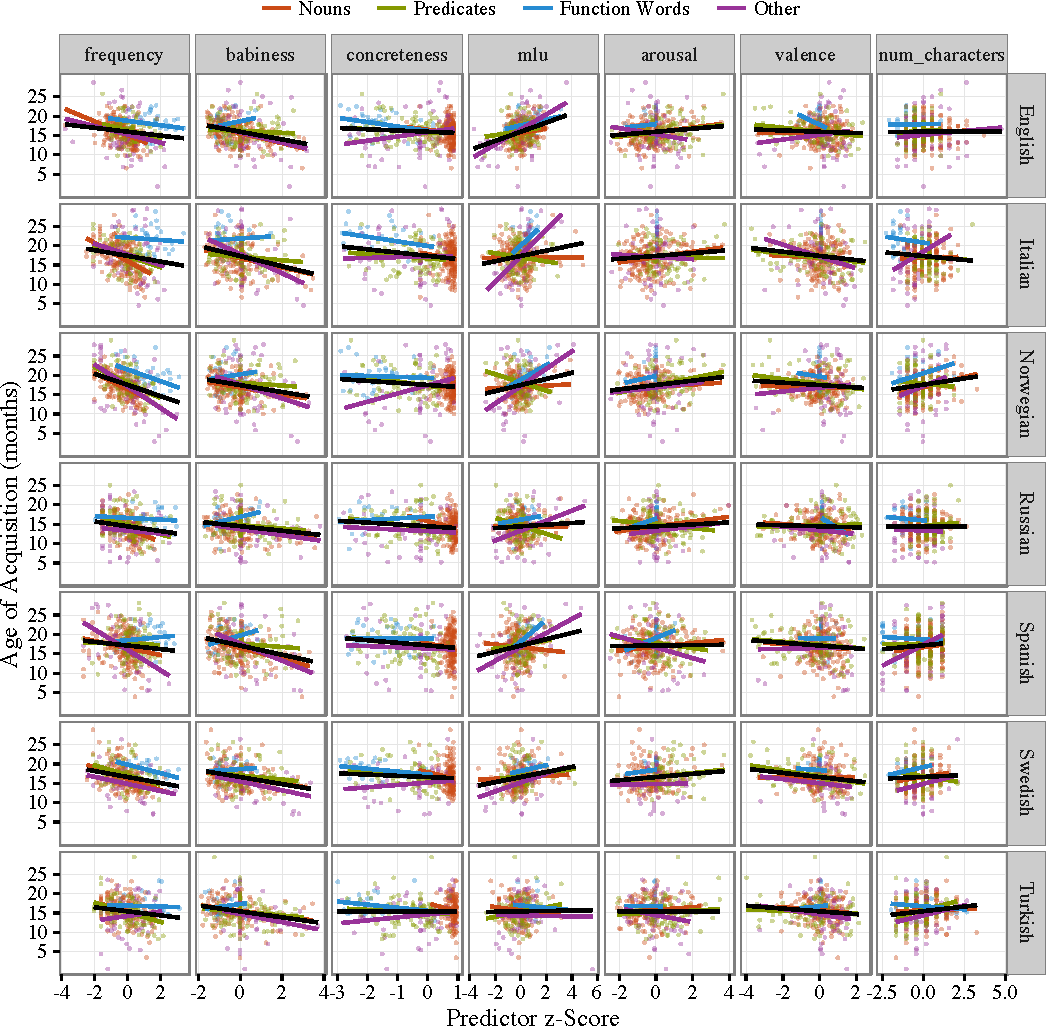
\includegraphics{figs/data-1} 

}

\caption[Relationship between predictors and AoA for each lexical category in each language]{Relationship between predictors and AoA for each lexical category in each language. Each point represents a word, with lines indicating linear model fits for each lexical category (in colors) and overall (in black).}\label{fig:data}
\end{figure*}
\end{CodeChunk}

\begin{CodeChunk}
\begin{figure*}[tb]

{\centering 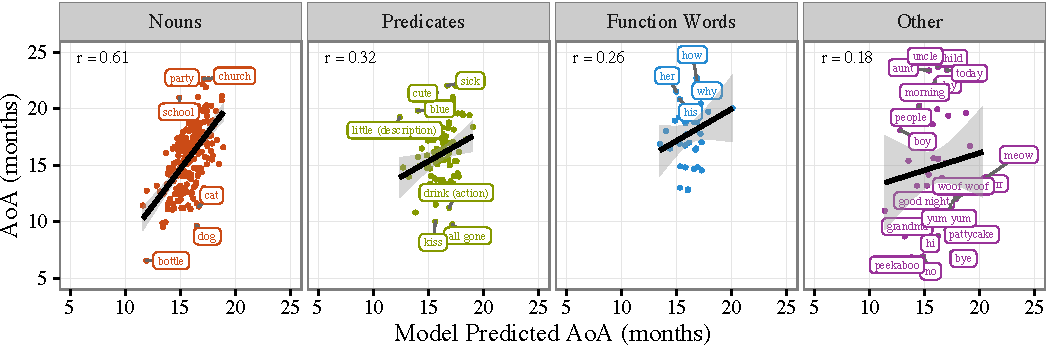
\includegraphics{figs/fit-1} 

}

\caption[Comparison between the model-predicted and actual ages of acquisition for words in English]{Comparison between the model-predicted and actual ages of acquisition for words in English. Words with an absolute error above 5 months are labelled for reference.}\label{fig:fit}
\end{figure*}
\end{CodeChunk}

\begin{CodeChunk}
\begin{figure}[!hb]

{\centering 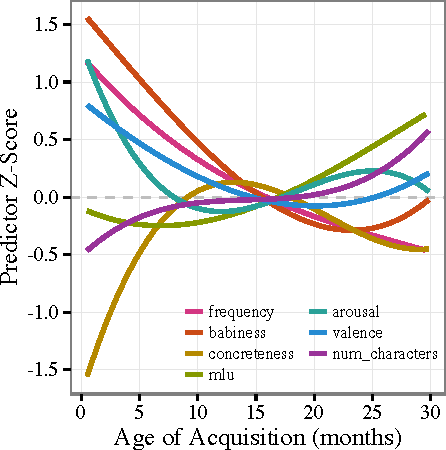
\includegraphics{figs/devo-1} 

}

\caption[Trends in predictor values across development (for all items in all languages)]{Trends in predictor values across development (for all items in all languages). Curves show best-fitting cubic regression.}\label{fig:devo}
\end{figure}
\end{CodeChunk}

\begin{CodeChunk}
\begin{figure*}[tb]

{\centering 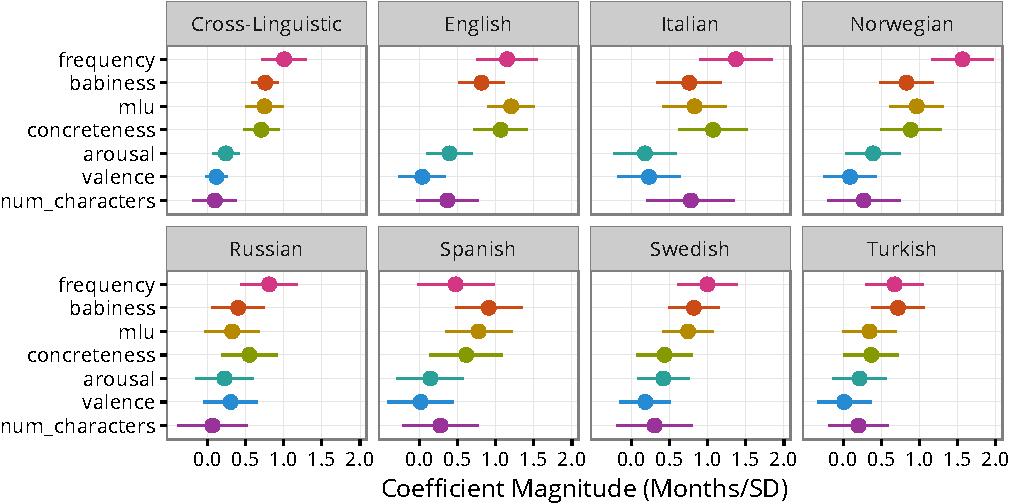
\includegraphics{figs/coefs-1} 

}

\caption[Estimates of predictor coefficients by language and for the all language model]{Estimates of predictor coefficients by language and for the all language model. Values above 0 indicate a positive relationship (i.e. words with higher MLU tend to have a higher AoA), while values below 0 indicate a negative relationship (i.e. words with higher frequency tend to have a lower AoA. Ranges indicate 95\% confidence intervals.}\label{fig:coefs}
\end{figure*}
\end{CodeChunk}

\begin{CodeChunk}
\begin{figure*}[tb]

{\centering 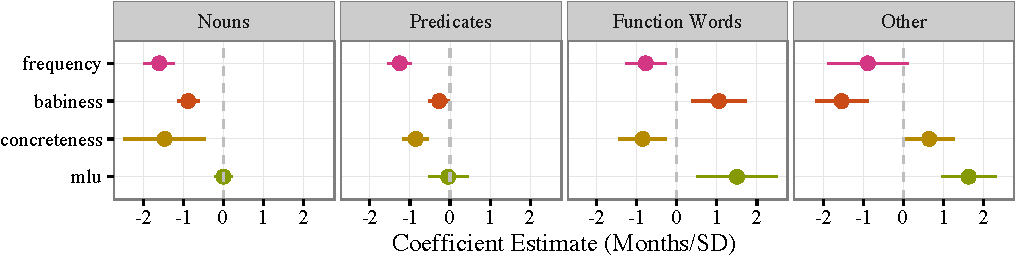
\includegraphics{figs/coefs_lexcat-1} 

}

\caption[Estimates of predictor coefficients by lexical category, without any separation by language and omitting the three weaker predictors]{Estimates of predictor coefficients by lexical category, without any separation by language and omitting the three weaker predictors. Ranges indicate 95\% confidence intervals.}\label{fig:coefs_lexcat}
\end{figure*}
\end{CodeChunk}

\subsection{Predictors}\label{predictors}

Each of our predictors is derived from independent sources. For each
word that appears on the CDI Word \& Gestures form in each of our seven
languages, we obtained an estimate of its frequency in child-directed
speech, the mean length of utterances in which it appears in
child-directed speech, its length in characters, and ratings of its
concreteness, valence, arousal, and relevance to babies. Items such as
\emph{child's own name} were excluded. Example words for these
predictors in English are shown in Table \ref{table:extremes}.

Frequency and MLU are measured relative to the word's language. But
since existing datasets for conceptual ratings are primarily available
for English, we mapped all words onto translation equivalents across CDI
forms, allowing us to use the ratings for English words across
languages. While necessarily imperfect, this method allows us to examine
languages for which limited resources exist. Translation equivalents are
available in the Wordbank database using the \texttt{wordbankr} package
in \texttt{R} (Frank et al., in press).

Each numeric predictor was centered and scaled so that all predictors
would have comparable units. Lexical category was determined on the
basis of the conceptual categories presented on the CDI form (e.g.,
``Animals''), such that the Nouns category contains common nouns,
Predicates contains verbs and adjectives, Function Words contains
closed-class words, and Other contains the remaining items (following
Bates et al., 1994).

\subsubsection{Frequency}\label{frequency}

For each language, we estimated word frequency from unigram counts based
on all corpora in CHILDES for that language. Each word's count includes
the counts of words that share the same stem (so that \emph{dogs} counts
as \emph{dog}) or are synonymous (so that \emph{father} counts as
\emph{daddy}). For polysemous word pairs (e.g., \emph{orange} as in
color or fruit), occurrences of the word in the corpus were split
uniformly between the senses on the CDI. Counts were normalized to the
length of each corpus and then log transformed.

\subsubsection{MLU}\label{mlu}

For each language, we estimated each word's MLU by calculating the mean
length in words of the utterances in which that word appeared, for all
corpora in CHILDES for that language. Words that only occurred in one
utterance were excluded.

\subsubsection{Length}\label{length}

We computed the number of characters in each word in each language.
While imperfect, this metric of length is highly correlated with number
of phonemes and syllables (Lewis \& Frank, under review).

\subsubsection{Concreteness}\label{concreteness}

We used previously collected norms for concreteness (Brysbaert,
Warriner, \& Kuperman, 2014), which were gathered by asking adult
participants to rate how concrete the meaning of each word is on a
5-point scale from abstract to concrete. For the 120 CDI words that were
not part of the collected norms, we imputed ratings from the mean of all
CDI words' ratings.

\subsubsection{Valence and Arousal}\label{valence-and-arousal}

We also used previously collected norms for valence and arousal
(Warriner, Kuperman, \& Brysbaert, 2013), for which adult participants
were asked to rate words on a 1-9 happy-unhappy scale (valence) and 1-9
excited-calm scale (arousal). For the 119 CDI words that were not part
of the collected norms (mostly function words), we imputed ratings from
the mean of all CDI words' ratings.

\subsubsection{Babiness}\label{babiness}

Lastly, we used previously collected norms of ``babiness,'' a measure of
association with infancy (Perry et al., 2015) for which adult
participants were asked to judge a word's relevance to babies.

\section{Analysis}\label{analysis}

An overview of our entire dataset can be seen in Figure \ref{fig:data},
which shows each word's estimated age of acquisition against its
predictor values, separated by language and lexical category. We present
three analyses of these data: 1) how predictor values change over
development, 2) their relative contributions to predicting AoA, and 3)
their interaction with lexical category.

\subsection{Developmental
Trajectories}\label{developmental-trajectories}

To assess developmental trends, we examine how the values of each
predictor change as a function of estimated AoA. Figure \ref{fig:devo}
shows these trajectories, with a cubic curve smoothing over all words.
Words that are learned earlier are more frequent, higher in babiness,
and appear in shorter utterances. Concreteness exhibits a U-shaped
trajectory, with the earliest learned words actually being relatively
abstract (e.g., social routines and animal sounds).

\subsection{Predicting AoA}\label{predicting-aoa}

We fit a linear regression for each language's data, as well as a linear
mixed-effects model with language as a random effect for all the data
pooled across languages. For illustrative purposes, Figure \ref{fig:fit}
shows the predictions of the English model plotted against the empirical
AoA estimates.

Figure \ref{fig:coefs} shows the coefficient estimate for each predictor
in each language and for all languages combined. We find that frequency,
babiness, concreteness, and MLU are relatively stronger predictors of
age of acquisition, across languages and in the full, cross-linguistic
model. Overall there is considerable consistency in how the predictors
pattern in various languages, although with some interesting
differences. For example, MLU in English appears to be unusually strong,
while frequency in Spanish looks unusually weak. There is also
variability in the overall fit of the models to the data, with some
languages (e.g., Norwegian), having much more of the variance explained
than others (e.g., Turkish).

A potential concern for comparing these coefficient estimates is
predictor collinearity. Fortunately, in every language, the only high
correlations were between frequency and number of characters, a
reflection of Zipf's Law (Zipf, 1935), and between frequency and
concreteness, probably as a consequence of the complexity bias (Lewis \&
Frank, under review).

\subsection{Lexical Category}\label{lexical-category}

Previous work gives reason to believe that predictors' relationship with
age of acquisition differs among various lexical categories (Goodman et
al., 2008). To investigate these effects, we separated our data by
lexical category and fit separate linear mixed-effects models for each,
limiting the predictors to the four that were significantly predictive
overall. Figure \ref{fig:coefs_lexcat} shows the resulting coefficient
estimates. Frequency matters most for nouns and comparatively little for
function words, while MLU is irrelevant for both nouns and predicates,
but highly informative for function words and other items.

\section{Discussion}\label{discussion}

What makes words easier or harder for young children to learn? Previous
experimental work has largely addressed this question using small-scale
experiments. While such experiments can identify sources of variation,
they typically do not allow for different sources to be compared in
detail. In contrast, observational studies allow the effects of
individual factors (with frequency being the most common) to be measured
across ages and lexical categories (e.g., Goodman et al., 2008). Scale
comes at a cost in terms of detail, however, since the availability of
both predictors and outcome data has been quite limited.

By including seven languages and as many predictors, our current work
expands the scope of previous observational studies of age of
acquisition. Our data show a number of patterns that confirm and expand
previous reports. First, predictors changed in relative importance
across development. For example, certain concepts that were more
strongly associated with babies appeared to be learned early for
children across languages (as in Tardif et al., 2008).

Second, we found general consistency in predictor coefficients across
languages (even as overall model fit varied, at least in part due to the
amount and quality of data for different languages). This consistency
supports the idea that differences in culture or language structure do
not lead to fundamentally different acquisition strategies, at least at
the level of detail we were able to examine.

Lastly, the predictors varied in strength across lexical categories.
Frequent, concrete nouns were learned earlier, consistent with theories
that emphasize the importance of early referential speech (e.g.,
Baldwin, 1995). But for predicates, concreteness was somewhat less
important, and for function words, MLU was most predictive. Overall
these findings are consistent with theories that emphasize the role of
linguistic structure over conceptual complexity in the acquisition of
other lexical categories beyond nouns (Gentner \& Boroditsky, 2001;
Snedeker et al., 2007).

Despite its larger scope, our work shares a number of important
limitations with previous studies. First and foremost, our approach is
to predict one set of individuals with data about the experience of a
completely different set and ratings of concepts gathered from yet
others. In contrast to dense-data analyses (B. C. Roy et al., 2015),
this approach fundamentally limits the amount of variability we will be
able to capture. In addition, the granularity of the predictors that can
be extracted from corpus data and applied to every word is necessarily
quite coarse. Ideally, predictors could be targeted more specifically at
particular theoretical constructs of interest (for example, the patterns
of use for specific predicates).

Finally, our work underscores the incompleteness of the current
understanding of vocabulary development. Even for English, the language
in which our model captures the most variance (\(r^2 = 0.29\)), much
still remains unexplained. Furthermore, this variance is highly
reliable---cross-validation using half of the English-speaking children
to predict ages of acquisition for the other half yields \(r^2 = 0.98\).
This gap highlights an important theoretical challenge in the study of
early language: linking individual datapoints to the broader patterns of
acquisition. We have strong theories of how individual learning
situations proceed, but must unify these theories to make progress on
understanding language learning at scale.

\vspace{1em}

\fbox{\parbox[b][][c]{7.3cm}{\centering All data and code for these analyses are available at\\ \url{https://github.com/mikabr/aoa-prediction}}}
\vspace{1em}

\section{Acknowledgements}\label{acknowledgements}

Thank you to Wordbank contributors and the MacArthur-Bates CDI Advisory
Board. This work supported by NSF BCS \#1528526.

\newpage

\section{References}\label{references}

\setlength{\parindent}{-0.1in} \setlength{\leftskip}{0.125in} \noindent

Baldwin, D. A. (1995). Understanding the link between joint attention
and language. \emph{Joint Attention: Its Origins and Role in
Development}, 131--158.

Bates, E., Marchman, V., Thal, D., Fenson, L., Dale, P., Reznick, J. S.,
\ldots{} Hartung, J. (1994). Developmental and stylistic variation in
the composition of early vocabulary. \emph{Journal of Child Language},
\emph{21}(01), 85--123.

Brysbaert, M., Warriner, A. B., \& Kuperman, V. (2014). Concreteness
ratings for 40 thousand generally known English word lemmas.
\emph{Behavior Research Methods}, \emph{46}(3), 904--911.

Fenson, L. (2007). \emph{MacArthur-Bates Communicative Development
Inventories: User's guide and technical manual}. Paul H. Brookes
Publishing Company.

Frank, M. C., Braginsky, M., Yurovsky, D., \& Marchman, V. A. (in
press). Wordbank: An open repository for developmental vocabulary data.
\emph{Journal of Child Language}.

Gentner, D., \& Boroditsky, L. (2001). Individuation, relativity, and
early word learning. In \emph{Language acquisition and conceptual
development}. Cambridge University Press.

Gleitman, L. (1990). The structural sources of verb meanings.
\emph{Language Acquisition}, \emph{1}(1), 3--55.

Goodman, J. C., Dale, P. S., \& Li, P. (2008). Does frequency count?
Parental input and the acquisition of vocabulary. \emph{Journal of Child
Language}, \emph{35}(3), 515.

Hills, T. T., Maouene, M., Maouene, J., Sheya, A., \& Smith, L. (2009).
Longitudinal analysis of early semantic networks: Preferential
attachment or preferential acquisition? \emph{Psychological Science},
\emph{20}(6), 729--739.

Lewis, M. L., \& Frank, M. C. (under review). The length of words
reflects their conceptual complexity.

MacWhinney, B. (2000). \emph{The CHILDES project: The database} (Vol.
2). Psychology Press.

Perry, L. K., Perlman, M., \& Lupyan, G. (2015). Iconicity in English
and Spanish and its relation to lexical category and age of acquisition.
\emph{PloS One}, \emph{10}(9), e0137147.

Roy, B. C., Frank, M. C., DeCamp, P., Miller, M., \& Roy, D. (2015).
Predicting the birth of a spoken word. \emph{Proceedings of the National
Academy of Sciences}, \emph{112}(41), 12663--12668.

Snedeker, J., Geren, J., \& Shafto, C. L. (2007). Starting over:
International adoption as a natural experiment in language development.
\emph{Psychological Science}, \emph{18}(1), 79--87.

Stokes, S. F. (2010). Neighborhood density and word frequency predict
vocabulary size in toddlers. \emph{Journal of Speech, Language, and
Hearing Research}, \emph{53}(3), 670--683.

Tardif, T., Fletcher, P., Liang, W., Zhang, Z., Kaciroti, N., \&
Marchman, V. A. (2008). Baby's first 10 words. \emph{Developmental
Psychology}, \emph{44}(4), 929.

Warriner, A. B., Kuperman, V., \& Brysbaert, M. (2013). Norms of
valence, arousal, and dominance for 13,915 English lemmas.
\emph{Behavior Research Methods}, \emph{45}(4), 1191--1207.

Zipf, G. K. (1935). The psycho-biology of language.

\end{document}
